\newpage
\section{Cell Selection}

\subsection{Introduction to Cells}

Our final product is a combination of muscle cells and oleogel-based fat substitute [https://www.nature.com/articles/s41467-023-38593-4]. Of the three muscle cell types (myocytes) found in vertebrates, beef is composed of skeletal muscle cells [https://www.ncbi.nlm.nih.gov/pmc/articles/PMC5167519/]. These cells can be derived from myoblasts through a process known as myogenesis, explained further in [SECTION DIFFERENTIATION]. 

[https://www.researchgate.net/figure/Myoblast-differentiation-Activated-satellite-cells-are-called-myoblasts-They-express_fig25_231588877] OR USE TRACEY’S FIGURE 4

The definition of a myoblast is “an undifferentiated cell capable of giving rise to muscle cells” [https://www.merriam-webster.com/dictionary/myoblast], which includes many different types of stem cells. When designing our cultured meat process, we need ensure our primary cells are suitable for both the process and final product. 

Myosatellite cells are the mode cell type used in industry, 23.1\% of 40 companies. [GFI-APAC-cell-line-survey-report-19-June-2023]

\subsection{Stem Cells}
We considered the following stem cell types for seeding our bioreactors:

\subsubsection*{Skeletal Muscle Stem Cells (Myosatellite)}
Under resting condition myosatellite cells are quiescent [dormant] and reside under the basal lamina [https://en.wikipedia.org/wiki/Basal_lamina] of the myofiber [https://www.sciencedirect.com/science/article/pii/B9780124160224000068?via\%3Dihub]. The overall myogenic differentiation pathway includes the activation of quiescent satellite cells, commitment to differentiation and proliferation, fusion to form myotubes, and ultimately maturation into myofibers.

\subsubsection*{Mesenchymal Stem Cells}
Mesenchymal stem cells (MSCs) are stromal cells that can self-renew. They are also capable of multilineage differentiation. MSCs can be isolated from a variety of tissues, such as umbilical cord, endometrial polyps, menses blood, bone marrow, adipose tissue, etc. [https://pubmed.ncbi.nlm.nih.gov/21396235/]. One of the major challenges is to elucidate the mechanisms of differentiation, mobilization, and homing of MSCs, which are highly complex.

\subsubsection*{Embryonic Stem Cells}
Embryonic stem cells (ESC) are obtained from the inner cell mass of the blastocyst and are associated with tumorigenesis [https://pubmed.ncbi.nlm.nih.gov/21396235/]. Embryonic stem cells are pluripotent meaning they can differentiate into all derivatives of the three primary germ layers. ESCs are capable of self-renewal in conditions that prevent differentiation and clumping. [https://www.science.org/doi/10.1126/science.282.5391.1145] [https://www.cell.com/cell/fulltext/S0092-8674\%2803\%2900847-X ]. ESCs have a shortened G1 phase and thus divide very frequently, allowing the cells to multiply quickly. ESCs have ethical considerations as harvesting embryonic stem cells usually necessitates destroying the embryo from which those cells are obtained.

\subsubsection*{Induced Pluripotent Stem Cell (iPSC)}
iPSCs can be obtained by reprogramming differentiated somatic cells. The genetic engineering required is high-cost due to its sensitivity, however base cell biopsy samples are easy to gain. Performance characteristics are similar to ESCs. [https://www.ncbi.nlm.nih.gov/pmc/articles/PMC3347549/] 

\subsection*{Other Cell Types}
The following cell types may be useful:

\subsubsection*{Fibroblast}
Fibroblast cells are used in the production of the extracellular matrix that can be used to provide texture to the meat. They can replicate indefinitely in vitro and are found in many parts of the body including skin. [https://www.ncbi.nlm.nih.gov/books/NBK26889/]

\subsubsection*{Adipocyte}
Adipocytes are the energy storage mechanism of the body, also known as fat cells. They are derived from Mesenchymal Stem Cells via adipogenesis. [https://www.ncbi.nlm.nih.gov/books/NBK555602/]

\begin{figure}[h]
    \centering
    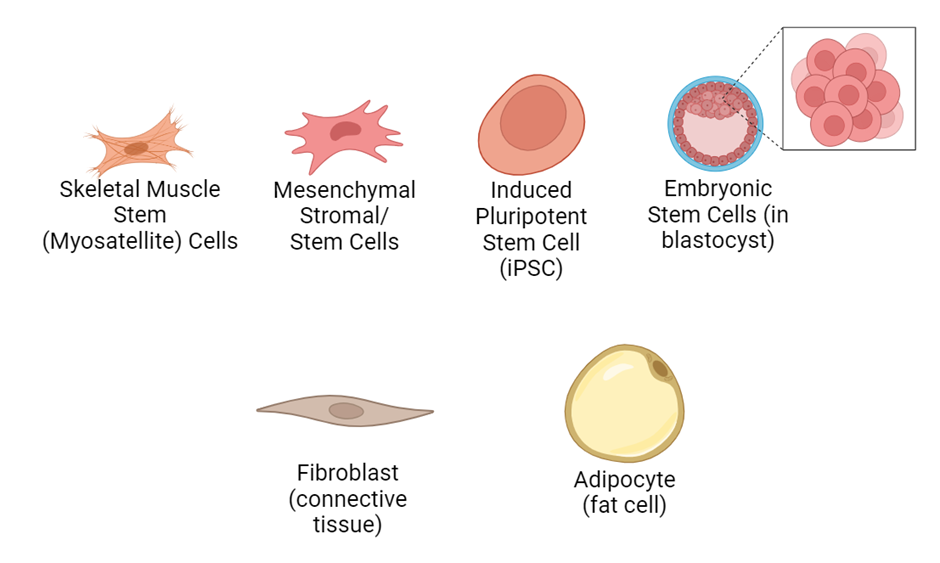
\includegraphics[width=0.75\textwidth]{will/w2i-cell-types.png}
    \hfill
    \caption{Cell types discussed, made in Biorender}
    \label{fig:cell-types}
\end{figure}

